\chapter{Desenvolupament del Projecte}
\label{chap:Desenvolupament}

L'objectiu del projecte és crear una plataforma per al desenvolupament de videojocs basada en els sistemes d'entitats. Aquesta plataforma ha de permetre la creació de diferents elements, com Components, Sistemes, Prototips, etc., que seran explicats en detall més endavant.
S'ha decidit que la millor manera de definir aquests elements és la de crear un llenguatge de programació que ho permeti. Aquest llenguatge s'anomenarà Quadriga, en honor a un dels esports amb més renom disputats als Jocs Olímpics clàssics.

En aquest capítol es parlarà primer del disseny del llenguatge en trets generals i s'entrarà en algun detall de la seva implementació. Seguidament es farà una introducció més detallada de les construccions pròpies del llenguatge i la seva funcionalitat. A continuació s'analitzarà el model de dades d'un programa compilat amb Quadriga i finalment es farà una petita introducció a les eines que s'han desenvolupat per tal d'ajudar la programació en Quadriga.

\section{Disseny i implementació}

  A la introducció, s'han descrit diferents aproximacions als sistemes d'entitats, i quines 5 característiques tindrà Quadriga. Aquí s'explica com s'ha intentat complir cada punt:

  \begin{itemize}
    \item {\bf Open Source} \hfill \\
      El codi del projecte s'ha penjat públicament a GoogleCode sota una llicència LGPL, que permet usar-la lliurement amb l'única restricció d'haver de publicar els canvis fets sobre la mateixa llibreria sota la mateixa llicència. També s'ha optat per fer servir només llibreries OpenSource com l'analitzador de sintaxi ({\em JavaCC}), la llibreria gràfica ({\em LWJGL}) i la base de dades ({\em HSQLDB}).
      
    \item {\bf Independent} \hfill \\
      S'ha optat per separar les {\em dades} de la funcionalitat, podent crear implementacions diferents per les mateixes dades, fent així que fins i tot puguem substituir tot el mòdul sencer de renderització (el motor gràfic) sense haver de tocar una línia de la definició de les entitats.
      
    \item {\bf Multi-plataforma de forma nativa} \hfill \\
      S'ha optat per programar sobre Java, i usar únicament llibreries escrites totalment amb Java o, en cas necessari, amb codi natiu multi-plataforma. S'intenta el màxim possible que no s'hagi de fer codi dependent de la plataforma.
      
    \item {\bf Permetre un desenvolupament ràpid un cop estiguin fets els components bàsics} \hfill \\
      S'ha intentat que la creació d'entitats i la seva interacció sigui el més senzilla possible.
      
    \item {\bf Fàcilment paral·lelitzable} \hfill \\
      S'han afegit expressament comportaments indefinits del programa, especialment en l'àmbit de l'ordre d'execució de certs elements, per exemple, d'ordre en que un sistema actualitza les entitats, o l'ordre en que 2 sistemes no relacionats s'actualitzen. D'aquesta manera es permet que el llenguatge mateix creï diferents fils d'execució i els balancegi de forma òptima.
  \end{itemize}

  Per tal de facilitar el disseny, s'ha decidit partir d'un parser de Java ja creat, en la seva versió 1.5, i modificar-lo de tal manera que admeti definicions noves i rebutgi aquelles que en Quadriga no tenen sentit, com són les classes.
  
  Podríem dir que s'ha modificat aquest parser tal que ara, en comptes de definir classes, es poden definir Components, Sistemes, Prototips, Events, Threads i objectes \"{}Main\"{}, que serviran com a punt d'inici de l'execució.
  
  A la figura \ref{fig:EsquemaExecucio} es pot veure un esquema bàsic sobre el recorregut teòric que un programa escrit en Quadriga segueix:
  
  \begin{figure}
    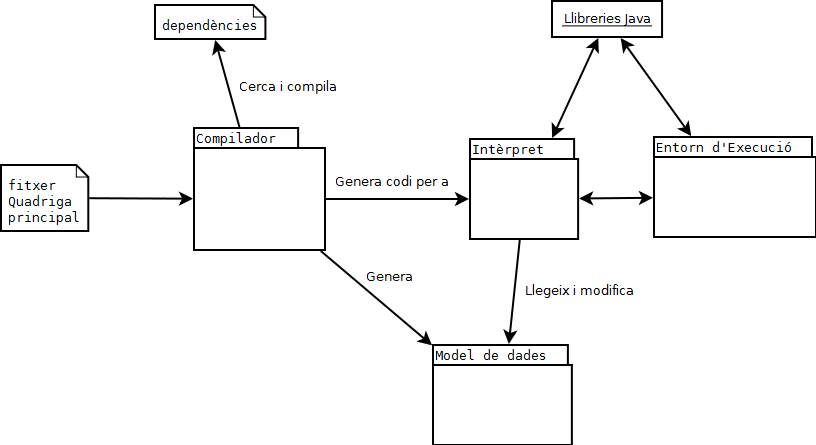
\includegraphics[width=1\linewidth]{./img/EsquemaExecucio.png}
    \caption{Esquema de l'execució \label{fig:EsquemaExecucio}}
  \end{figure}
  
  \begin{enumerate}
    \item Es crida l'execució de Quadriga passant-li per paràmetre l'objecte de tipus Main que volem executar, i en quin fitxer es troba.
    \item El programa compila aquest fitxer i cerca quines dependències té. Cerca i compila aquestes dependències.
    \item Un cop compilat el programa, es crea un model de dades especial per a aquest, que depèn dels components definits, ja que per cada un d'aquests s'han de guardar unes dades diferents.
    \item Tenint el model de dades i un codi executable, l'intèrpret carrega les llibreries que necessita i executa aquest codi, que treballa sobre el model de dades creat.
  \end{enumerate}
  
  A la figura \ref{fig:DiagramaDeModuls} es mostren de forma més detallada els mòduls del programa i les seves interconnexions.

  \begin{figure}
    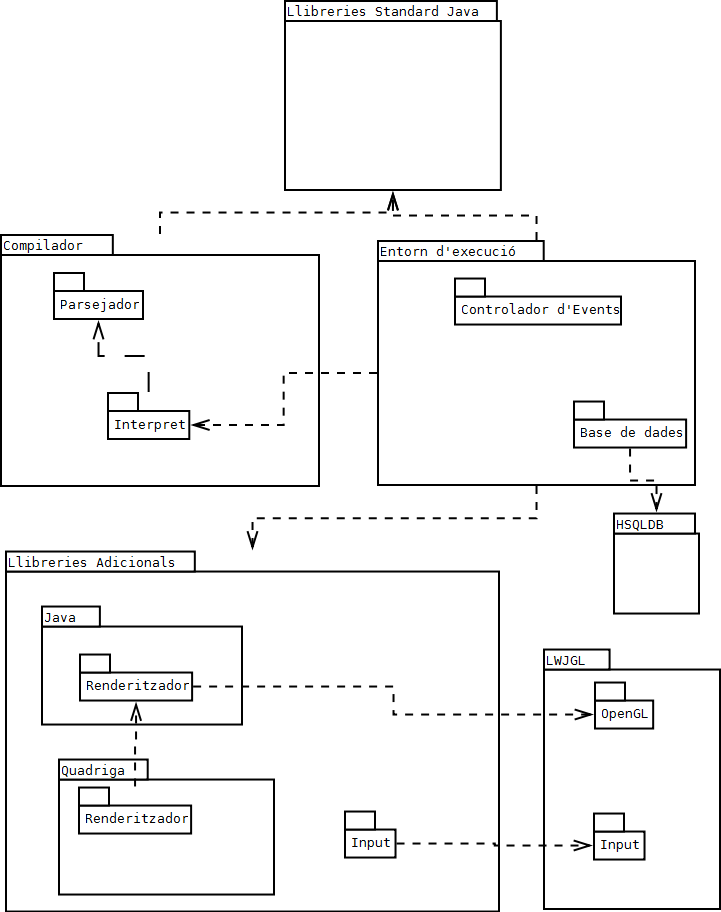
\includegraphics[width=1\linewidth]{./img/Moduls.png}
    \caption{Diagrama de mòduls \label{fig:DiagramaDeModuls}}
  \end{figure}
  
\section{Definicions pròpies del llenguatge Quadriga}

  Aquí s'explicaran les definicions bàsiques de conceptes propis del Sistema d'entitats Quadriga. Per a més informació consultar \cite{EntityWikiB} o \cite{Martin07}, llocs d'on he tret la inspiració bàsica per crear aquest sistema.

  Essencialment es tracta de crear una API idèntica a una Base de Dades relacional on:

  \begin{itemize}
    \item Les claus primàries són les \"{}Entitats\"{}
    \item Cada fila és un array de dades, anomenat \"{}Component\"{}
    \item Cada taula està associada a un \"{}Component\"{}
  \end{itemize}

  A continuació es detallen les definicions, element a element:
  
  \begin{itemize}
    \item{\bf Entitat}

      En un nivell molt concret, una entitat és simplement un enter, o identificador, únic. A nivell més abstracte, una entitat és tot aquell objecte que apareix d'alguna manera en un joc.
      
      En general, qualsevol element del joc pot ser una entitat. Des de l'escenari, o parts de l'escenari, a l'avatar del jugador, cada enemic o PNJ (personatge no jugador), ítems, etc... Fins i tot poden haver entitats més abstractes, que creïn els programadors, com una entitat que representi un nivell, o la GUI (Graphical User Interface), o fins i tot un diàleg.

      Quadriga no permet definir un tipus de dades \"{}Entitat\"{} en sí, sinó ja la té definida com a tipus bàsic i permet d'instanciar-ne de noves, eliminar-les, afegir i treure components i aplicar-li prototips (explicats més endavant).
      
      També és important introduir la idea de que les entitats formen una jerarquia en forma d'arbre. Per exemple podem crear un personatge capaç de dur diverses armes. Sabem que les armes sempre s'hauran de veure a la mà d'aquest personatge, per tal de fer-ho, indiquem que l'arma duta pel personatge és filla d'aquest a la jerarquia.
      
    \item{\bf Component}

      Un component és un conjunt de dades que defineixen l'estat d'una entitat. Hi ha diferents tipus de components i cada un aporta diferents dades. Cada component també du associada certa funcionalitat, però aquesta mai es troba dintre del mateix component, sinó en un sistema (tenint sempre una separació de codi i dades, molt semblant l'esquema Model-View-Controller).
      
      Com a exemples tindríem: Transformació de l'objecte (la translació i rotació que un objecte té respecte l'origen del món), Objecte animat (component que indica quin model s'ha d'utilitzar per a renderitzar l'entitat, que a més pot contenir informació de quines animacions té, etc...), Component de IA que indicaria quines coses sap l'entitat tal que el sistema o mòdul de IA pot fer servir per a prendre decisions, etc\ldots
      
      Per a definir un component, Quadriga permet d'assignar-li un identificador i la llista de dades que contindrà. Addicionalment es permet de llistar requisits, o sigui, altres components que prèviament una entitat necessita tenir per tal de poder tenir aquest.
      
    \item{\bf Event}

      Un event, o esdeveniment, és un objecte que serveix per a passar missatges entre entitats. Aquests events són llençats quan succeeix alguna cosa (un event d'input, o un sistema que en llença un) i pot ser tractat per un o més sistemes. Els events es poden llençar a una entitat concreta o fer un broadcast a totes les entitats.
      
      Exemples en tindríem: cada possible ordre que el jugador dóna al joc; com moure's cap a endavant, disparar, activar un ordinador\ldots També podríem tenir events per indicar-li a una entitat que ha estat impactada per una bala, o que li diguessin que ha mort, de tal manera que es pugui activar la animació corresponent, etc\ldots

      Un event es declara a Quadriga de forma molt similar a un Component. Només cal indicar-ne el nom i quina informació aportarà.

    \item{\bf Sistema}

      Un Sistema és un Objecte opac que s'encarrega d'una part de la funcionalitat del joc, per exemple:
      \begin{itemize}
        \item{\bf Physics System} s'activa cada 17ms i itera sobre totes les entitats amb física i fa un frame de simulació.
        \item{\bf Rendering System} itera sobre totes les entitats amb representació 2D/3D i les renderitza per pantalla.
        \item{\bf Script System} itera sobre totes les entitats que tenen un script associat i crida aquest script.
      \end{itemize}

      Un sistema sap sobre quines entitats ha d'iterar en saber quins components té associada cada entitat. Per exemple el sistema de física iterarà sobre totes aquelles entitats que tinguin algun component que descrigui informació física, i no tocarà cap altra entitat.

      La creació d'un sistema en Quadriga és la més complexa: cal especificar-li un identificador i sobre quin tipus d'entitats actua, o sigui, quins components han de tenir entitats. Després permet declarar un seguit de funcions que entren en quatre categories bàsiques:
      
      \begin{enumerate}
        \item {\bf Creació i destrucció d'entitats:} Es cridaran cada cop que una entitat aparegui per primera o última vegada, respectivament, entre les entitats afectades per aquest sistema.
        \item {\bf Actualització d'entitats:} Es cridarà cada tick del joc.
        \item {\bf Events:} Permet especificar una funció per cada tipus d'Event, que es cridarà cada vegada que una entitat pertanyent al sistema sigui afectada per aquest event.
        \item {\bf Inicialització i neteja del sistema:} Es cridaran una vegada a l'inici i final de l'execució del programa.
      \end{enumerate}
      
    \item{\bf Thread}

      Un Thread és una agrupació de sistemes que s'han d'executar en un ordre establert, seguint així unes garanties.
      
      Normalment agrupen els sistemes de formes temàtiques: Thread de IA, Thread de física, Thread de renderitzar, Thread de lògica, etc\ldots
      
      Per especificar un Thread en Quadriga cal indicar-ne el nom, quins sistemes contindrà (l'ordre és important) i a més permet crear mètodes d'inicialització i finalització que es cridaran a l'inici i al final de l'execució del programa.

    \item{\bf Prototip}

      Un prototip és una eina que ajuda a crear entitats. Conceptualment és semblant a una funció que insereix els components necessaris amb els paràmetres que toquen per crear-la. És, com el seu nom indica, el prototip d'un tipus d'entitats.
      
      Un exemple força típic és tenir un prototip per a cada tipus d'enemic del joc, i a l'hora de crear els enemics d'un nivell s'indica de quin tipus són i s'afegeix informació concreta de cada instància: com la posició, el grup al qual pertanyen, etc\ldots És molt important remarcar que els prototips només serveixen per crear entitats i aquestes no recorden quin prototip les ha instanciat.
      
      La creació d'un prototip en Quadriga és similar a la creació d'una funció, on s'especifica component a component com es construeix una entitat. A més permet de crear altres entitats \"{}filles\"{}, tal que es pugui crear un subarbre d'entitats cridant un sol prototip.

    \item{\bf Main}

      L'Objecte Main defineix quins threads executa l'aplicació i una funció d'inicialització de la mateixa. Quan s'executa un programa Quadriga, s'ha d'especificar el nom d'un objecte tipus Main per a executar.
    
      Un Main es declara a Quadriga indicant quins Threads ha de crear, i afegint funcions d'inicialització i finalització.
    
  \end{itemize}
  
  Per a més informació sobre el llenguatge en sí, consultar l'apèndix \ref{chap:llenguatgeQ}.

\section{Model de Dades}

  Com ja s'ha comentat, un sistema d'entitats acaba sent molt semblant a una Base de Dades relacional, on cada tipus de component equival a una taula, cada entitat a un identificador i en cada fila d'aquestes taules hi ha les dades corresponents. A més, aquesta base de dades ha de complir un seguit d'especificacions:

  \begin{itemize}
    \item Els sistemes d'entitats consten de 4 elements bàsics: entitats, components, sistemes i events.
    
    \item Cada entitat és única i té un identificador únic. A més, pot tenir informació de Debug.
      \begin{itemize}
        \item Cada entitat pot tenir una entitat Pare associada, de manera que es pugui fer un graf amb les entitats (que sempre tindrà forma d'arbre).
        \item Cada entitat pot tenir un nom associat.
        \item Cada parella pare-nom equivaldrà a una única entitat.
      \end{itemize}
    \item Cada component tindrà el seu nom i un identificador únic.
    
    \item Cada sistema tindrà el seu nom i un identificador únic.
    
    \item Cada event tindrà el seu nom i un identificador únic.
    
    \item Cada sistema s'ha d'associar amb els components i events als quals afecta.
    
    \item Cada sistema haurà de guardar un registre de totes les entitats a les que ha afectat en la darrera iteració del joc.
    
    \item Quan un component s'associa a una entitat, es crea una instància d'aquest component i se'n guarden les dades.
    
    \item Cada tipus de component té unes dades associades diferents que es programen mitjançant el llenguatge Quadriga.
  \end{itemize}

  L'esquema Entiat-Relació resultant es mostra a la figura \ref{fig:EntitatRelacio}. I la base de dades relacional tindria la forma mostrada a la figura \ref{fig:BBDDRelacional}.

  \begin{figure}
    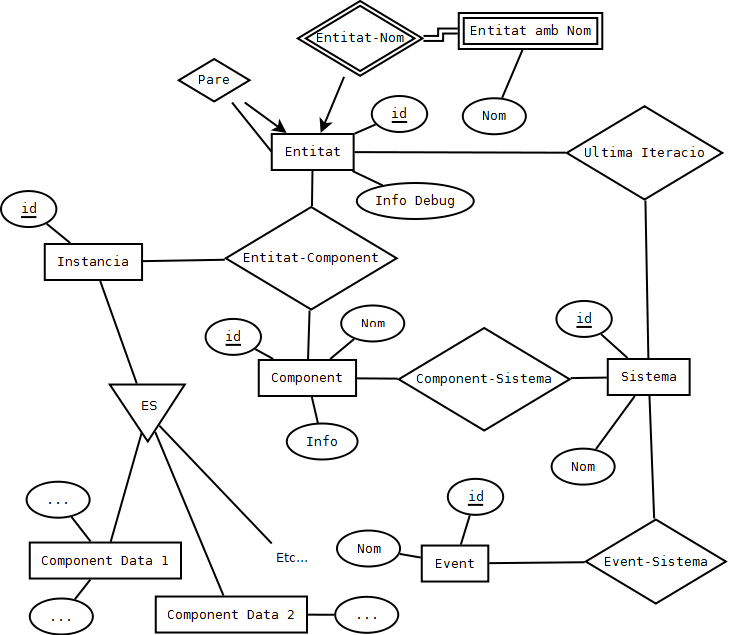
\includegraphics[width=1\linewidth]{./img/EntitatRelacio.png}
    \caption{Model Enitat-Relació \label{fig:EntitatRelacio}}
  \end{figure}

  \begin{figure}
    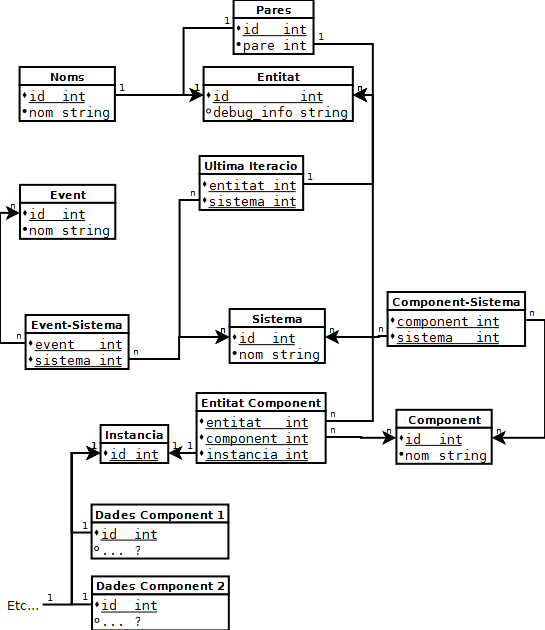
\includegraphics[width=1\linewidth]{./img/BBDDRelacional.png}
    \caption{Base de dades. \label{fig:BBDDRelacional}}
  \end{figure}
  
  Cal destacar en aquest apartat, que el model serà lleugerament diferent per cada programa compilat amb Quadriga, doncs es generarà una taula addicional per a cada component descrit, amb els camps corresponents. No serà la mateixa base de dades per un joc simple, estil {\em Tetris}, que per un MMORPG estil {\em World of Warcraft}, tal i com la intuïció ens fa saber.
  
  La implementació d'aquesta base de dades s'ha optat per fer-la amb un motor SQL per a Java anomenat {\em HSQLDB}. Això ens proporciona eines com les cerques optimitzades i facilitats de guardar i carregar la base de dades de forma molt senzilla, però a canvi es perd força rendiment respecte si la base de dades es fes de forma més específica.

\section{Editar el llenguatge}

  Per tal de facilitar l'edició de {\em Quadriga} s'ha implementat un senzill plug-in per a {\em Notepad++} que es pot descarregar des de \url{http://code.google.com/p/quadriga/downloads/detail?name=quadriga.xml} i importar al mateix {\em Notepad++}. No és tan complert com podria ser un editor d'una IDE, amb auto-completat i subratllament d'errors i advertències, sinó que simplement marca les paraules claus i els operadors per a fer una petita ajuda visual.